\PassOptionsToPackage{unicode=true}{hyperref} % options for packages loaded elsewhere
\PassOptionsToPackage{hyphens}{url}
\PassOptionsToPackage{dvipsnames,svgnames*,x11names*}{xcolor}
%
\documentclass[]{article}
\usepackage{lmodern}
\usepackage{amssymb,amsmath}
\usepackage{ifxetex,ifluatex}
\usepackage{fixltx2e} % provides \textsubscript
\ifnum 0\ifxetex 1\fi\ifluatex 1\fi=0 % if pdftex
  \usepackage[T1]{fontenc}
  \usepackage[utf8]{inputenc}
  \usepackage{textcomp} % provides euro and other symbols
\else % if luatex or xelatex
  \usepackage{unicode-math}
  \defaultfontfeatures{Ligatures=TeX,Scale=MatchLowercase}
\fi
% use upquote if available, for straight quotes in verbatim environments
\IfFileExists{upquote.sty}{\usepackage{upquote}}{}
% use microtype if available
\IfFileExists{microtype.sty}{%
\usepackage[]{microtype}
\UseMicrotypeSet[protrusion]{basicmath} % disable protrusion for tt fonts
}{}
\IfFileExists{parskip.sty}{%
\usepackage{parskip}
}{% else
\setlength{\parindent}{0pt}
\setlength{\parskip}{6pt plus 2pt minus 1pt}
}
\usepackage{xcolor}
\usepackage{hyperref}
\hypersetup{
            pdftitle={Week 2 - Homework},
            pdfauthor={Omar Boffil},
            colorlinks=true,
            linkcolor=Maroon,
            filecolor=Maroon,
            citecolor=Blue,
            urlcolor=cyan,
            breaklinks=true}
\urlstyle{same}  % don't use monospace font for urls
\usepackage[margin=1in]{geometry}
\usepackage{color}
\usepackage{fancyvrb}
\newcommand{\VerbBar}{|}
\newcommand{\VERB}{\Verb[commandchars=\\\{\}]}
\DefineVerbatimEnvironment{Highlighting}{Verbatim}{commandchars=\\\{\}}
% Add ',fontsize=\small' for more characters per line
\usepackage{framed}
\definecolor{shadecolor}{RGB}{248,248,248}
\newenvironment{Shaded}{\begin{snugshade}}{\end{snugshade}}
\newcommand{\AlertTok}[1]{\textcolor[rgb]{0.94,0.16,0.16}{#1}}
\newcommand{\AnnotationTok}[1]{\textcolor[rgb]{0.56,0.35,0.01}{\textbf{\textit{#1}}}}
\newcommand{\AttributeTok}[1]{\textcolor[rgb]{0.77,0.63,0.00}{#1}}
\newcommand{\BaseNTok}[1]{\textcolor[rgb]{0.00,0.00,0.81}{#1}}
\newcommand{\BuiltInTok}[1]{#1}
\newcommand{\CharTok}[1]{\textcolor[rgb]{0.31,0.60,0.02}{#1}}
\newcommand{\CommentTok}[1]{\textcolor[rgb]{0.56,0.35,0.01}{\textit{#1}}}
\newcommand{\CommentVarTok}[1]{\textcolor[rgb]{0.56,0.35,0.01}{\textbf{\textit{#1}}}}
\newcommand{\ConstantTok}[1]{\textcolor[rgb]{0.00,0.00,0.00}{#1}}
\newcommand{\ControlFlowTok}[1]{\textcolor[rgb]{0.13,0.29,0.53}{\textbf{#1}}}
\newcommand{\DataTypeTok}[1]{\textcolor[rgb]{0.13,0.29,0.53}{#1}}
\newcommand{\DecValTok}[1]{\textcolor[rgb]{0.00,0.00,0.81}{#1}}
\newcommand{\DocumentationTok}[1]{\textcolor[rgb]{0.56,0.35,0.01}{\textbf{\textit{#1}}}}
\newcommand{\ErrorTok}[1]{\textcolor[rgb]{0.64,0.00,0.00}{\textbf{#1}}}
\newcommand{\ExtensionTok}[1]{#1}
\newcommand{\FloatTok}[1]{\textcolor[rgb]{0.00,0.00,0.81}{#1}}
\newcommand{\FunctionTok}[1]{\textcolor[rgb]{0.00,0.00,0.00}{#1}}
\newcommand{\ImportTok}[1]{#1}
\newcommand{\InformationTok}[1]{\textcolor[rgb]{0.56,0.35,0.01}{\textbf{\textit{#1}}}}
\newcommand{\KeywordTok}[1]{\textcolor[rgb]{0.13,0.29,0.53}{\textbf{#1}}}
\newcommand{\NormalTok}[1]{#1}
\newcommand{\OperatorTok}[1]{\textcolor[rgb]{0.81,0.36,0.00}{\textbf{#1}}}
\newcommand{\OtherTok}[1]{\textcolor[rgb]{0.56,0.35,0.01}{#1}}
\newcommand{\PreprocessorTok}[1]{\textcolor[rgb]{0.56,0.35,0.01}{\textit{#1}}}
\newcommand{\RegionMarkerTok}[1]{#1}
\newcommand{\SpecialCharTok}[1]{\textcolor[rgb]{0.00,0.00,0.00}{#1}}
\newcommand{\SpecialStringTok}[1]{\textcolor[rgb]{0.31,0.60,0.02}{#1}}
\newcommand{\StringTok}[1]{\textcolor[rgb]{0.31,0.60,0.02}{#1}}
\newcommand{\VariableTok}[1]{\textcolor[rgb]{0.00,0.00,0.00}{#1}}
\newcommand{\VerbatimStringTok}[1]{\textcolor[rgb]{0.31,0.60,0.02}{#1}}
\newcommand{\WarningTok}[1]{\textcolor[rgb]{0.56,0.35,0.01}{\textbf{\textit{#1}}}}
\usepackage{longtable,booktabs}
% Fix footnotes in tables (requires footnote package)
\IfFileExists{footnote.sty}{\usepackage{footnote}\makesavenoteenv{longtable}}{}
\usepackage{graphicx,grffile}
\makeatletter
\def\maxwidth{\ifdim\Gin@nat@width>\linewidth\linewidth\else\Gin@nat@width\fi}
\def\maxheight{\ifdim\Gin@nat@height>\textheight\textheight\else\Gin@nat@height\fi}
\makeatother
% Scale images if necessary, so that they will not overflow the page
% margins by default, and it is still possible to overwrite the defaults
% using explicit options in \includegraphics[width, height, ...]{}
\setkeys{Gin}{width=\maxwidth,height=\maxheight,keepaspectratio}
\setlength{\emergencystretch}{3em}  % prevent overfull lines
\providecommand{\tightlist}{%
  \setlength{\itemsep}{0pt}\setlength{\parskip}{0pt}}
\setcounter{secnumdepth}{0}
% Redefines (sub)paragraphs to behave more like sections
\ifx\paragraph\undefined\else
\let\oldparagraph\paragraph
\renewcommand{\paragraph}[1]{\oldparagraph{#1}\mbox{}}
\fi
\ifx\subparagraph\undefined\else
\let\oldsubparagraph\subparagraph
\renewcommand{\subparagraph}[1]{\oldsubparagraph{#1}\mbox{}}
\fi

% set default figure placement to htbp
\makeatletter
\def\fps@figure{htbp}
\makeatother


\title{Week 2 - Homework}
\author{Omar Boffil}
\date{05/30/2020}

\begin{document}
\maketitle

\begin{center}\rule{0.5\linewidth}{0.5pt}\end{center}

\hypertarget{exercise-1-using-lm}{%
\subsection{\texorpdfstring{Exercise 1 (Using
\texttt{lm})}{Exercise 1 (Using lm)}}\label{exercise-1-using-lm}}

For this exercise we will use the \texttt{cats} dataset from the
\texttt{MASS} package. You should use \texttt{?cats} to learn about the
background of this dataset.

\textbf{(a)} Suppose we would like to understand the size of a cat's
heart based on the body weight of a cat. Fit a simple linear model in
\texttt{R} that accomplishes this task. Store the results in a variable
called \texttt{cat\_model}. Output the result of calling
\texttt{summary()} on \texttt{cat\_model}.

\begin{Shaded}
\begin{Highlighting}[]
\KeywordTok{library}\NormalTok{(MASS)}
\NormalTok{body =}\StringTok{ }\NormalTok{cats}\OperatorTok{$}\NormalTok{Bwt}
\NormalTok{heart =}\StringTok{ }\NormalTok{cats}\OperatorTok{$}\NormalTok{Hwt}
\NormalTok{cat_model =}\StringTok{ }\KeywordTok{lm}\NormalTok{(heart }\OperatorTok{~}\StringTok{ }\NormalTok{body, }\DataTypeTok{data =}\NormalTok{ cats)}
\KeywordTok{summary}\NormalTok{(cat_model)}
\end{Highlighting}
\end{Shaded}

\begin{verbatim}
## 
## Call:
## lm(formula = heart ~ body, data = cats)
## 
## Residuals:
##     Min      1Q  Median      3Q     Max 
## -3.5694 -0.9634 -0.0921  1.0426  5.1238 
## 
## Coefficients:
##             Estimate Std. Error t value Pr(>|t|)    
## (Intercept)  -0.3567     0.6923  -0.515    0.607    
## body          4.0341     0.2503  16.119   <2e-16 ***
## ---
## Signif. codes:  0 '***' 0.001 '**' 0.01 '*' 0.05 '.' 0.1 ' ' 1
## 
## Residual standard error: 1.452 on 142 degrees of freedom
## Multiple R-squared:  0.6466, Adjusted R-squared:  0.6441 
## F-statistic: 259.8 on 1 and 142 DF,  p-value: < 2.2e-16
\end{verbatim}

\textbf{(b)} Output only the estimated regression coefficients.
Interpret \(\hat{\beta_0}\) and \(\beta_1\) in the \emph{context of the
problem}. Be aware that only one of those is an estimate.

\begin{Shaded}
\begin{Highlighting}[]
\NormalTok{cat_model}\OperatorTok{$}\NormalTok{coefficients}
\end{Highlighting}
\end{Shaded}

\begin{verbatim}
## (Intercept)        body 
##  -0.3566624   4.0340627
\end{verbatim}

\(\hat{\beta_1}\) of 4.0341 g is the estimated increase in mean for the
cat's heart weight to the rise of 1 kg cat weight.

\(\hat{\beta_0}\) is -0.3566624 g is the estimate mean cat's heart
weight for a cat of 0 kg weight

\textbf{(c)} Use your model to predict the heart weight of a cat that
weights \textbf{3.1} kg. Do you feel confident in this prediction?
Briefly explain.

\begin{Shaded}
\begin{Highlighting}[]
\KeywordTok{predict}\NormalTok{(cat_model, }\DataTypeTok{newdata =} \KeywordTok{data.frame}\NormalTok{(}\DataTypeTok{body =} \FloatTok{3.1}\NormalTok{))}
\end{Highlighting}
\end{Shaded}

\begin{verbatim}
##        1 
## 12.14893
\end{verbatim}

Yes, I feel confident because it is close to the mean which is 12.5

\textbf{(d)} Use your model to predict the heart weight of a cat that
weights \textbf{1.5} kg. Do you feel confident in this prediction?
Briefly explain.

\begin{Shaded}
\begin{Highlighting}[]
\KeywordTok{predict}\NormalTok{(cat_model, }\DataTypeTok{newdata =} \KeywordTok{data.frame}\NormalTok{(}\DataTypeTok{body =} \FloatTok{1.5}\NormalTok{))}
\end{Highlighting}
\end{Shaded}

\begin{verbatim}
##        1 
## 5.694432
\end{verbatim}

Yes, because the values is close to the mean for that value

\textbf{(e)} Create a scatterplot of the data and add the fitted
regression line. Make sure your plot is well labeled and is somewhat
visually appealing.

\begin{Shaded}
\begin{Highlighting}[]
\KeywordTok{plot}\NormalTok{(heart }\OperatorTok{~}\StringTok{ }\NormalTok{body, }\DataTypeTok{data =}\NormalTok{ cats, }\DataTypeTok{main =} \StringTok{"Cat's heart weight based on the body weight"}\NormalTok{,}
     \DataTypeTok{xlab =} \StringTok{"Body weight"}\NormalTok{, }\DataTypeTok{ylab =} \StringTok{"Heart weight"}\NormalTok{, }\DataTypeTok{col =} \StringTok{"red"}\NormalTok{, }\DataTypeTok{pch  =} \DecValTok{20} 
\NormalTok{     )}

\KeywordTok{abline}\NormalTok{(}\KeywordTok{lm}\NormalTok{(heart }\OperatorTok{~}\StringTok{ }\NormalTok{body, }\DataTypeTok{data =}\NormalTok{ cats), }\DataTypeTok{col =} \StringTok{"blue"}\NormalTok{)}
\end{Highlighting}
\end{Shaded}

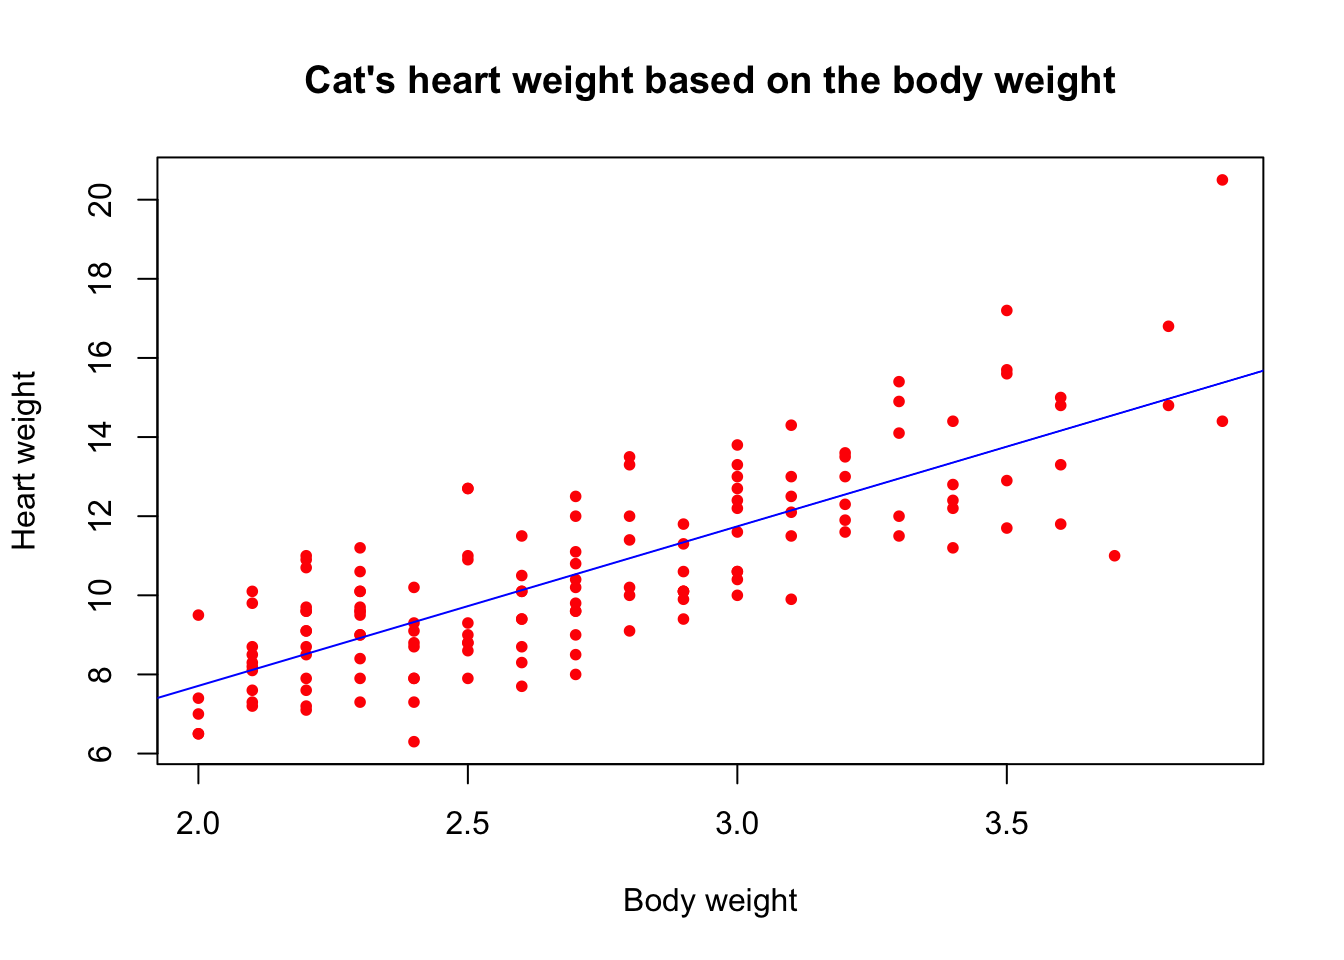
\includegraphics{w02-hw-oboffil2_files/figure-latex/unnamed-chunk-5-1.pdf}

\textbf{(f)} Report the value of \(R^2\) for the model. Do so directly.
Do not simply copy and paste the value from the full output in the
console after running \texttt{summary()} in part \textbf{(a)}.

\(R^2\) is 0.6466209

\begin{center}\rule{0.5\linewidth}{0.5pt}\end{center}

\hypertarget{exercise-2-writing-functions}{%
\subsection{Exercise 2 (Writing
Functions)}\label{exercise-2-writing-functions}}

This exercise is a continuation of Exercise 1.

\textbf{(a)} Write a function called \texttt{get\_sd\_est} that
calculates an estimate of \(\sigma\) in one of two ways depending on
input to the function. The function should take three arguments as
input:

\begin{itemize}
\tightlist
\item
  \texttt{fitted\_vals} - A vector of fitted values from a model
\item
  \texttt{actual\_vals} - A vector of the true values of the response
\item
  \texttt{mle} - A logical (\texttt{TRUE} / \texttt{FALSE}) variable
  which defaults to \texttt{FALSE}
\end{itemize}

The function should return a single value:

\begin{itemize}
\tightlist
\item
  \(s_e\) if \texttt{mle} is set to \texttt{FALSE}.
\item
  \(\hat{\sigma}\) if \texttt{mle} is set to \texttt{TRUE}.
\end{itemize}

\begin{Shaded}
\begin{Highlighting}[]
\NormalTok{get_sd_est =}\StringTok{ }\ControlFlowTok{function}\NormalTok{(fitted_vals, actual_vals, }\DataTypeTok{mle =} \OtherTok{FALSE}\NormalTok{)\{}
  
  \ControlFlowTok{if}\NormalTok{ (mle }\OperatorTok{==}\StringTok{ }\OtherTok{FALSE}\NormalTok{)\{}
    \KeywordTok{summary}\NormalTok{(fitted_vals)}\OperatorTok{$}\NormalTok{sigma}
\NormalTok{  \}}\ControlFlowTok{else}\NormalTok{\{}
    \KeywordTok{sd}\NormalTok{(actual_vals }\OperatorTok{-}\StringTok{ }\KeywordTok{mean}\NormalTok{(actual_vals)) }
\NormalTok{  \}}
  
\NormalTok{\}}
\end{Highlighting}
\end{Shaded}

\textbf{(b)} Run the function \texttt{get\_sd\_est} on the residuals
from the model in Exercise 1, with \texttt{mle} set to \texttt{FALSE}.
Explain the resulting estimate in the context of the model.

\begin{Shaded}
\begin{Highlighting}[]
\KeywordTok{get_sd_est}\NormalTok{(cat_model, cats}\OperatorTok{$}\NormalTok{Hwt, }\OtherTok{FALSE}\NormalTok{)}
\end{Highlighting}
\end{Shaded}

\begin{verbatim}
## [1] 1.452373
\end{verbatim}

\textbf{(c)} Run the function \texttt{get\_sd\_est} on the residuals
from the model in Exercise 1, with \texttt{mle} set to \texttt{TRUE}.
Explain the resulting estimate in the context of the model. Note that we
are trying to estimate the same parameter as in part \textbf{(b)}.

\begin{Shaded}
\begin{Highlighting}[]
\KeywordTok{get_sd_est}\NormalTok{(cat_model, cats}\OperatorTok{$}\NormalTok{Hwt, }\OtherTok{TRUE}\NormalTok{)}
\end{Highlighting}
\end{Shaded}

\begin{verbatim}
## [1] 2.434636
\end{verbatim}

\textbf{(d)} To check your work, output
\texttt{summary(cat\_model)\$sigma}. It should match at least one of
\textbf{(b)} or \textbf{(c)}.

\begin{Shaded}
\begin{Highlighting}[]
\KeywordTok{all.equal}\NormalTok{(}\KeywordTok{get_sd_est}\NormalTok{(cat_model, cats}\OperatorTok{$}\NormalTok{Hwt, }\OtherTok{FALSE}\NormalTok{), }\KeywordTok{summary}\NormalTok{(cat_model)}\OperatorTok{$}\NormalTok{sigma)}
\end{Highlighting}
\end{Shaded}

\begin{verbatim}
## [1] TRUE
\end{verbatim}

\begin{Shaded}
\begin{Highlighting}[]
\KeywordTok{all.equal}\NormalTok{(}\KeywordTok{get_sd_est}\NormalTok{(cat_model, cats}\OperatorTok{$}\NormalTok{Hwt, }\OtherTok{TRUE}\NormalTok{), }\KeywordTok{summary}\NormalTok{(cat_model)}\OperatorTok{$}\NormalTok{sigma)}
\end{Highlighting}
\end{Shaded}

\begin{verbatim}
## [1] "Mean relative difference: 0.4034535"
\end{verbatim}

\begin{center}\rule{0.5\linewidth}{0.5pt}\end{center}

\hypertarget{exercise-3-simulating-slr}{%
\subsection{Exercise 3 (Simulating
SLR)}\label{exercise-3-simulating-slr}}

Consider the model

\[
Y_i = 5 + -3 x_i + \epsilon_i
\]

with

\[
\epsilon_i \sim N(\mu = 0, \sigma^2 = 10.24)
\]

where \(\beta_0 = 5\) and \(\beta_1 = -3\).

This exercise relies heavily on generating random observations. To make
this reproducible we will set a seed for the randomization. Alter the
following code to make \texttt{birthday} store your birthday in the
format: \texttt{yyyymmdd}. For example,
\href{https://en.wikipedia.org/wiki/William_Sealy_Gosset}{William
Gosset}, better known as \emph{Student}, was born on June 13, 1876, so
he would use:

\begin{Shaded}
\begin{Highlighting}[]
\NormalTok{birthday =}\StringTok{ }\DecValTok{19900826}
\KeywordTok{set.seed}\NormalTok{(birthday)}
\end{Highlighting}
\end{Shaded}

\textbf{(a)} Use \texttt{R} to simulate \texttt{n\ =\ 25} observations
from the above model. For the remainder of this exercise, use the
following ``known'' values of \(x\).

\begin{Shaded}
\begin{Highlighting}[]
\NormalTok{num_obs =}\StringTok{ }\DecValTok{25}
\NormalTok{beta_}\DecValTok{0}\NormalTok{ =}\StringTok{ }\DecValTok{5}
\NormalTok{beta_}\DecValTok{1}\NormalTok{ =}\StringTok{ }\DecValTok{-3}
\NormalTok{sigma =}\StringTok{ }\KeywordTok{sqrt}\NormalTok{(}\FloatTok{10.24}\NormalTok{)}
\KeywordTok{set.seed}\NormalTok{(}\DecValTok{2}\NormalTok{)}
\NormalTok{above =}\StringTok{ }\KeywordTok{rnorm}\NormalTok{(}\DecValTok{25}\NormalTok{, }\DecValTok{0}\NormalTok{, sigma)}
\NormalTok{above}
\end{Highlighting}
\end{Shaded}

\begin{verbatim}
##  [1] -2.87012655  0.59151739  5.08110506 -3.61720216 -0.25680562  0.42374491
##  [7]  2.26545513 -0.76703368  6.35031660 -0.44411844  1.33648240  3.14160889
## [13] -1.25662514 -3.32694073  5.70313267 -7.39542107  2.81153466  0.11458150
## [19]  3.24105181  1.38324849  6.69062146 -3.83976262  5.08684224  6.25488526
## [25]  0.01580089
\end{verbatim}

\begin{Shaded}
\begin{Highlighting}[]
\KeywordTok{set.seed}\NormalTok{(}\DecValTok{1}\NormalTok{)}
\NormalTok{x =}\StringTok{ }\KeywordTok{runif}\NormalTok{(}\DataTypeTok{n =} \DecValTok{25}\NormalTok{, }\DecValTok{0}\NormalTok{, }\DecValTok{10}\NormalTok{)}
\end{Highlighting}
\end{Shaded}

You may use
\href{http://daviddalpiaz.github.io/appliedstats/simple-linear-regression.html\#simulating-slr}{the
\texttt{sim\_slr} function provided in the text}. Store the data frame
this function returns in a variable of your choice. Note that this
function calls \(y\) \texttt{response} and \(x\) \texttt{predictor}.

\textbf{(b)} Fit a model to your simulated data. Report the estimated
coefficients. Are they close to what you would expect? Briefly explain.

\begin{Shaded}
\begin{Highlighting}[]
\NormalTok{y =}\StringTok{ }\NormalTok{beta_}\DecValTok{0} \OperatorTok{+}\StringTok{ }\NormalTok{beta_}\DecValTok{1} \OperatorTok{*}\StringTok{ }\NormalTok{x }\OperatorTok{+}\StringTok{ }\NormalTok{above}
\NormalTok{df_fit =}\StringTok{ }\KeywordTok{lm}\NormalTok{(y }\OperatorTok{~}\StringTok{ }\NormalTok{x)}
\KeywordTok{coef}\NormalTok{(df_fit)}
\end{Highlighting}
\end{Shaded}

\begin{verbatim}
## (Intercept)           x 
##    4.998661   -2.798781
\end{verbatim}

The coefficients are what I expect they are close in value to the actual
parameters

\textbf{(c)} Plot the data you simulated in part \textbf{(a)}. Add the
regression line from part \textbf{(b)} as well as the line for the true
model. Hint: Keep all plotting commands in the same chunk.

\begin{Shaded}
\begin{Highlighting}[]
\KeywordTok{plot}\NormalTok{(y }\OperatorTok{~}\StringTok{ }\NormalTok{x, }\DataTypeTok{main =} \StringTok{"Simulated Regression Data"}\NormalTok{,}
     \DataTypeTok{xlab =} \StringTok{"Predictor"}\NormalTok{,}
     \DataTypeTok{ylab =} \StringTok{"Response"}\NormalTok{)}
\KeywordTok{abline}\NormalTok{(df_fit, }\DataTypeTok{col =} \StringTok{"blue"}\NormalTok{)}
\KeywordTok{abline}\NormalTok{(beta_}\DecValTok{0}\NormalTok{, beta_}\DecValTok{1}\NormalTok{, }\DataTypeTok{lty =} \DecValTok{2}\NormalTok{, }\DataTypeTok{col =} \StringTok{"red"}\NormalTok{)}
\KeywordTok{legend}\NormalTok{(}\StringTok{"topright"}\NormalTok{, }\KeywordTok{c}\NormalTok{(}\StringTok{"Estimate"}\NormalTok{, }\StringTok{"Truth"}\NormalTok{), }\DataTypeTok{lty =} \KeywordTok{c}\NormalTok{(}\DecValTok{1}\NormalTok{, }\DecValTok{2}\NormalTok{), }\DataTypeTok{lwd =} \DecValTok{2}\NormalTok{, }\DataTypeTok{col =} \KeywordTok{c}\NormalTok{(}\StringTok{"blue"}\NormalTok{, }\StringTok{"red"}\NormalTok{))}
\end{Highlighting}
\end{Shaded}

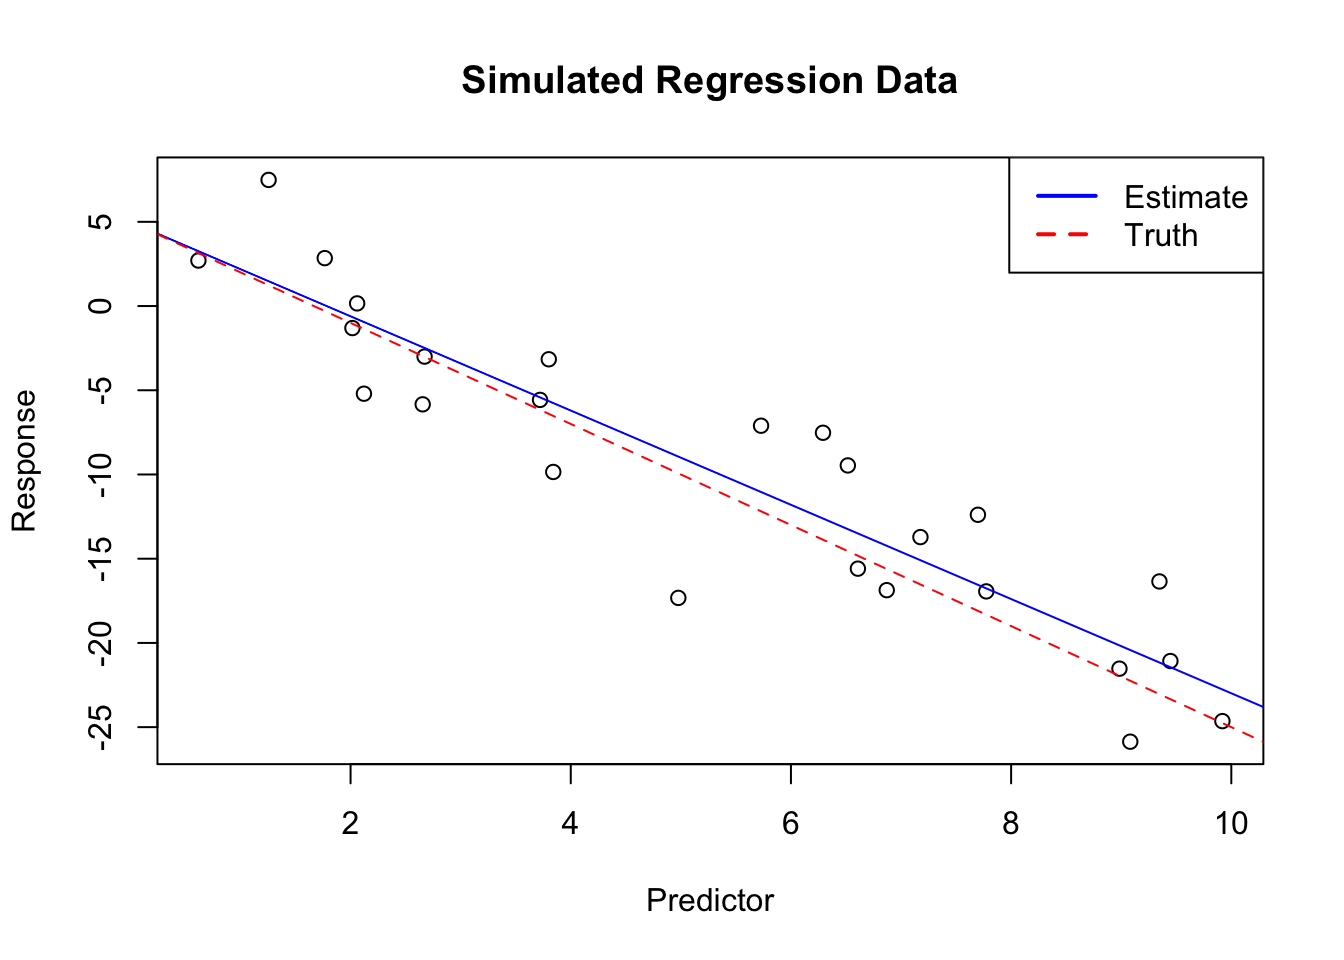
\includegraphics{w02-hw-oboffil2_files/figure-latex/unnamed-chunk-13-1.pdf}

\textbf{(d)} Use \texttt{R} to repeat the process of simulating
\texttt{n\ =\ 25} observations from the above model \(1500\) times. Each
time fit a SLR model to the data and store the value of
\(\hat{\beta_1}\) in a variable called \texttt{beta\_hat\_1}. Some
hints:

\begin{itemize}
\tightlist
\item
  Consider a \texttt{for} loop.
\item
  Create \texttt{beta\_hat\_1} before writing the \texttt{for} loop.
  Make it a vector of length \(1500\) where each element is \texttt{0}.
\item
  Inside the body of the \texttt{for} loop, simulate new \(y\) data each
  time. Use a variable to temporarily store this data together with the
  known \(x\) data as a data frame.
\item
  After simulating the data, use \texttt{lm()} to fit a regression. Use
  a variable to temporarily store this output.
\item
  Use the \texttt{coef()} function and \texttt{{[}{]}} to extract the
  correct estimated coefficient.
\item
  Use \texttt{beta\_hat\_1{[}i{]}} to store in elements of
  \texttt{beta\_hat\_1}.
\item
  See the notes on
  \href{http://daviddalpiaz.github.io/appliedstats/introduction-to-r.html\#distribution-of-a-sample-mean}{Distribution
  of a Sample Mean} for some inspiration.
\end{itemize}

You can do this differently if you like. Use of these hints is not
required.

\begin{Shaded}
\begin{Highlighting}[]
\NormalTok{beta_hat_}\DecValTok{1}\NormalTok{ =}\StringTok{ }\KeywordTok{c}\NormalTok{(}\KeywordTok{rep}\NormalTok{(}\DecValTok{0}\NormalTok{,}\DecValTok{1500}\NormalTok{))}

\ControlFlowTok{for}\NormalTok{ (i }\ControlFlowTok{in} \DecValTok{1}\OperatorTok{:}\DecValTok{1500}\NormalTok{) \{}
  
\NormalTok{  above =}\StringTok{ }\KeywordTok{rnorm}\NormalTok{(}\DecValTok{25}\NormalTok{, }\DecValTok{0}\NormalTok{, sigma)}
\NormalTok{  x =}\StringTok{ }\KeywordTok{runif}\NormalTok{(}\DataTypeTok{n =} \DecValTok{25}\NormalTok{, }\DecValTok{0}\NormalTok{, }\DecValTok{10}\NormalTok{)}
\NormalTok{  y =}\StringTok{ }\NormalTok{beta_}\DecValTok{0} \OperatorTok{+}\StringTok{ }\NormalTok{beta_}\DecValTok{1} \OperatorTok{*}\StringTok{ }\NormalTok{x }\OperatorTok{+}\StringTok{ }\NormalTok{above}
\NormalTok{  df_fit =}\StringTok{ }\KeywordTok{lm}\NormalTok{(y }\OperatorTok{~}\StringTok{ }\NormalTok{x)}
  
\NormalTok{  beta_hat_}\DecValTok{1}\NormalTok{[i] =}\StringTok{ }\KeywordTok{coef}\NormalTok{(df_fit)[}\DecValTok{2}\NormalTok{]}
\NormalTok{\}}
\end{Highlighting}
\end{Shaded}

\textbf{(e)} Report the mean and standard deviation of
\texttt{beta\_hat\_1}. Do either of these look familiar?

Mean of \(\hat{\beta_1}\) is: -3.0046894 Standard deviation of
\(\hat{\beta_1}\) is: 0.2340423

Yes, values look familiar especially the mean that is equal to the
\{\beta\_1\}

\textbf{(f)} Plot a histogram of \texttt{beta\_hat\_1}. Comment on the
shape of this histogram.

\begin{Shaded}
\begin{Highlighting}[]
\KeywordTok{hist}\NormalTok{(beta_hat_}\DecValTok{1}\NormalTok{)}
\end{Highlighting}
\end{Shaded}

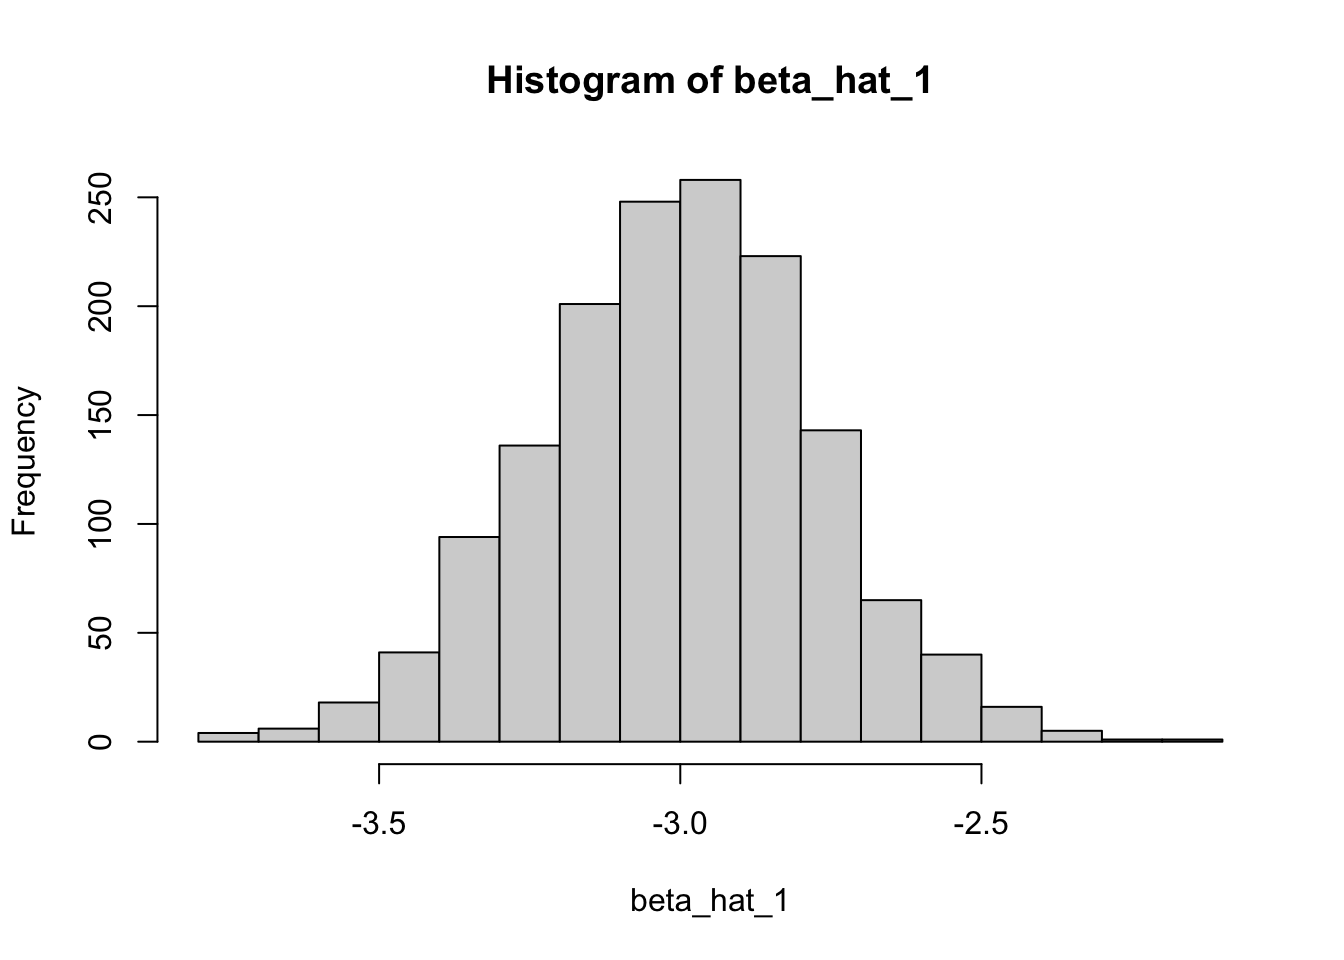
\includegraphics{w02-hw-oboffil2_files/figure-latex/unnamed-chunk-15-1.pdf}
The shape is Symmetry meaning that the media and the mean are equal or
very close

\begin{center}\rule{0.5\linewidth}{0.5pt}\end{center}

\hypertarget{exercise-4-be-a-skeptic}{%
\subsection{Exercise 4 (Be a Skeptic)}\label{exercise-4-be-a-skeptic}}

Consider the model

\[
Y_i = 3 + 0 \cdot x_i + \epsilon_i
\]

with

\[
\epsilon_i \sim N(\mu = 0, \sigma^2 = 4)
\]

where \(\beta_0 = 3\) and \(\beta_1 = 0\).

Before answering the following parts, set a seed value equal to
\textbf{your} birthday, as was done in the previous exercise.

\begin{Shaded}
\begin{Highlighting}[]
\NormalTok{birthday =}\StringTok{ }\DecValTok{19900826}
\KeywordTok{set.seed}\NormalTok{(birthday)}
\end{Highlighting}
\end{Shaded}

\textbf{(a)} Use \texttt{R} to repeat the process of simulating
\texttt{n\ =\ 75} observations from the above model \(2500\) times. For
the remainder of this exercise, use the following ``known'' values of
\(x\).

\begin{Shaded}
\begin{Highlighting}[]
\NormalTok{beta_}\DecValTok{0}\NormalTok{ =}\StringTok{ }\DecValTok{3}
\NormalTok{beta_}\DecValTok{1}\NormalTok{ =}\StringTok{ }\DecValTok{0}
\NormalTok{sigma =}\StringTok{ }\KeywordTok{sqrt}\NormalTok{(}\DecValTok{4}\NormalTok{)}
\NormalTok{beta_hat_}\DecValTok{1}\NormalTok{ =}\StringTok{ }\KeywordTok{c}\NormalTok{(}\KeywordTok{rep}\NormalTok{(}\DecValTok{0}\NormalTok{, }\DecValTok{2500}\NormalTok{))}

\ControlFlowTok{for}\NormalTok{ (i }\ControlFlowTok{in} \DecValTok{1}\OperatorTok{:}\DecValTok{2500}\NormalTok{)\{}
\NormalTok{  above =}\StringTok{ }\KeywordTok{rnorm}\NormalTok{(}\DecValTok{75}\NormalTok{, }\DecValTok{0}\NormalTok{, sigma)}
\NormalTok{  x =}\StringTok{ }\KeywordTok{runif}\NormalTok{(}\DataTypeTok{n =} \DecValTok{75}\NormalTok{, }\DecValTok{0}\NormalTok{, }\DecValTok{10}\NormalTok{)}
\NormalTok{  y =}\StringTok{ }\NormalTok{beta_}\DecValTok{0} \OperatorTok{+}\StringTok{ }\NormalTok{beta_}\DecValTok{1} \OperatorTok{*}\StringTok{ }\NormalTok{x }\OperatorTok{+}\StringTok{ }\NormalTok{above}
\NormalTok{  df_fit =}\StringTok{ }\KeywordTok{lm}\NormalTok{(y }\OperatorTok{~}\StringTok{ }\NormalTok{x)}
\NormalTok{  beta_hat_}\DecValTok{1}\NormalTok{[i] =}\StringTok{ }\KeywordTok{coef}\NormalTok{(df_fit)[}\DecValTok{2}\NormalTok{]}
\NormalTok{\}}
\end{Highlighting}
\end{Shaded}

Each time fit a SLR model to the data and store the value of
\(\hat{\beta_1}\) in a variable called \texttt{beta\_hat\_1}. You may
use
\href{http://daviddalpiaz.github.io/appliedstats/simple-linear-regression.html\#simulating-slr}{the
\texttt{sim\_slr} function provided in the text}. Hint: Yes
\(\beta_1 = 0\).

\textbf{(b)} Plot a histogram of \texttt{beta\_hat\_1}. Comment on the
shape of this histogram.

\begin{Shaded}
\begin{Highlighting}[]
\KeywordTok{hist}\NormalTok{(beta_hat_}\DecValTok{1}\NormalTok{)}
\end{Highlighting}
\end{Shaded}

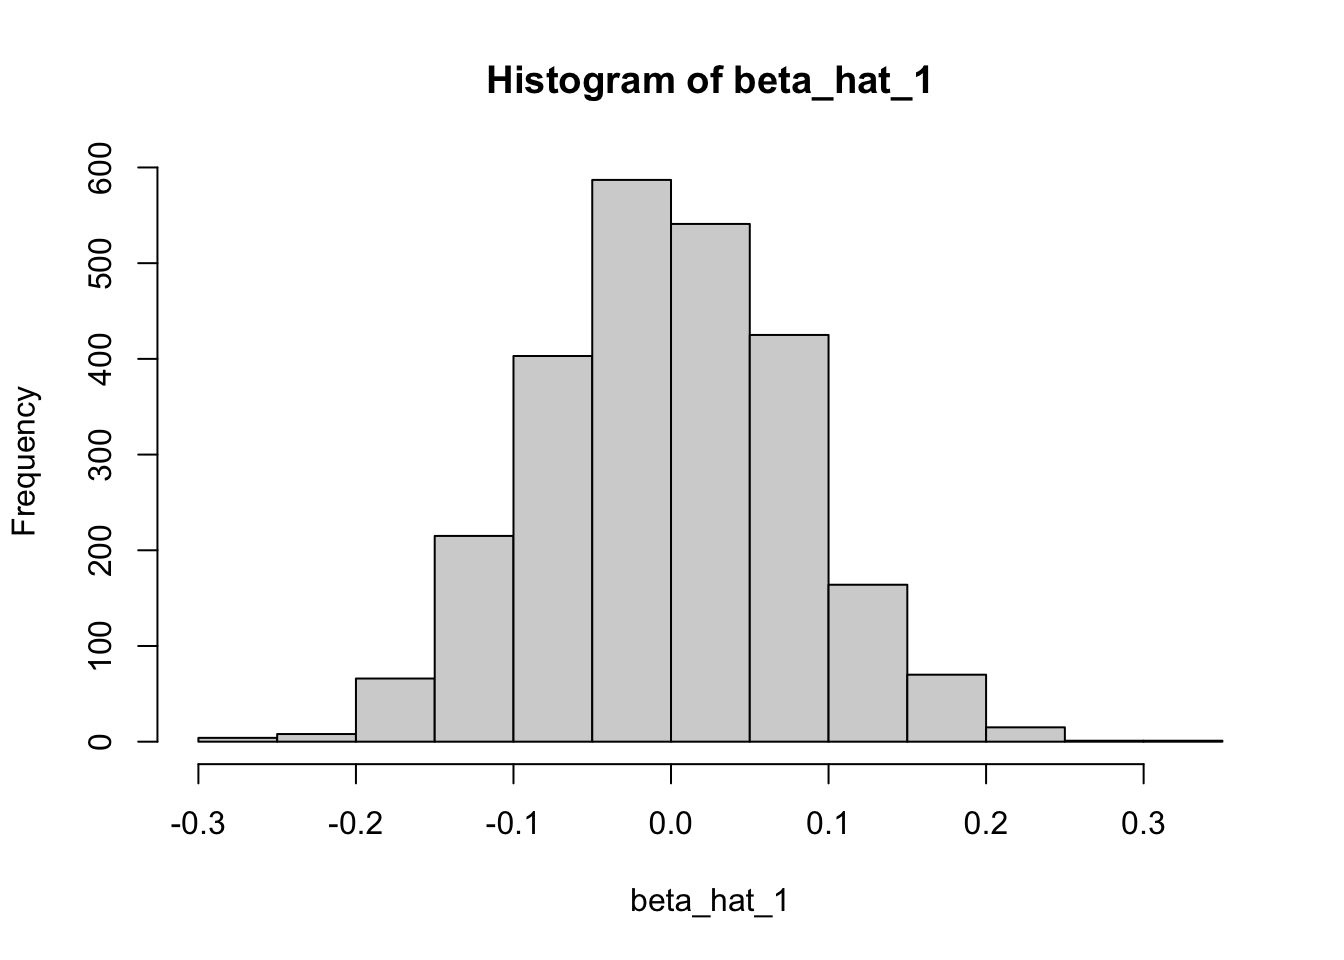
\includegraphics{w02-hw-oboffil2_files/figure-latex/unnamed-chunk-18-1.pdf}

The majority of the data are on the left side the Histogram skewed to
the right because the mean is higher than the media

\textbf{(c)} Import the data in \href{skeptic.csv}{\texttt{skeptic.csv}}
and fit a SLR model. The variable names in \texttt{skeptic.csv} follow
the same convention as those returned by \texttt{sim\_slr()}. Extract
the fitted coefficient for \(\beta_1\).

\begin{Shaded}
\begin{Highlighting}[]
\KeywordTok{library}\NormalTok{(readr)}
\NormalTok{skeptic =}\StringTok{ }\KeywordTok{read_csv}\NormalTok{(}\StringTok{"skeptic.csv"}\NormalTok{, }
    \DataTypeTok{col_types =} \KeywordTok{cols}\NormalTok{(}\DataTypeTok{predictor =} \KeywordTok{col_double}\NormalTok{(), }
        \DataTypeTok{response =} \KeywordTok{col_double}\NormalTok{()))}
\end{Highlighting}
\end{Shaded}

\begin{Shaded}
\begin{Highlighting}[]
\NormalTok{skeptic_df =}\StringTok{ }\KeywordTok{lm}\NormalTok{(skeptic}\OperatorTok{$}\NormalTok{response }\OperatorTok{~}\StringTok{ }\NormalTok{skeptic}\OperatorTok{$}\NormalTok{predictor, skeptic)}
\NormalTok{beta_}\DecValTok{1}\NormalTok{_hat_skeptic =}\StringTok{ }\KeywordTok{coef}\NormalTok{(skeptic_df)[}\DecValTok{2}\NormalTok{]}
\NormalTok{beta_}\DecValTok{1}\NormalTok{_hat_skeptic}
\end{Highlighting}
\end{Shaded}

\begin{verbatim}
## skeptic$predictor 
##        -0.2221927
\end{verbatim}

\textbf{(d)} Re-plot the histogram from \textbf{(b)}. Now add a vertical
red line at the value of \(\hat{\beta_1}\) in part \textbf{(c)}. To do
so, you'll need to use \texttt{abline(v\ =\ c,\ col\ =\ "red")} where
\texttt{c} is your value.

\begin{Shaded}
\begin{Highlighting}[]
\KeywordTok{hist}\NormalTok{(beta_hat_}\DecValTok{1}\NormalTok{)}
\KeywordTok{abline}\NormalTok{(}\DataTypeTok{v =}\NormalTok{ beta_}\DecValTok{1}\NormalTok{_hat_skeptic, }\DataTypeTok{col =} \StringTok{"red"}\NormalTok{)}
\end{Highlighting}
\end{Shaded}

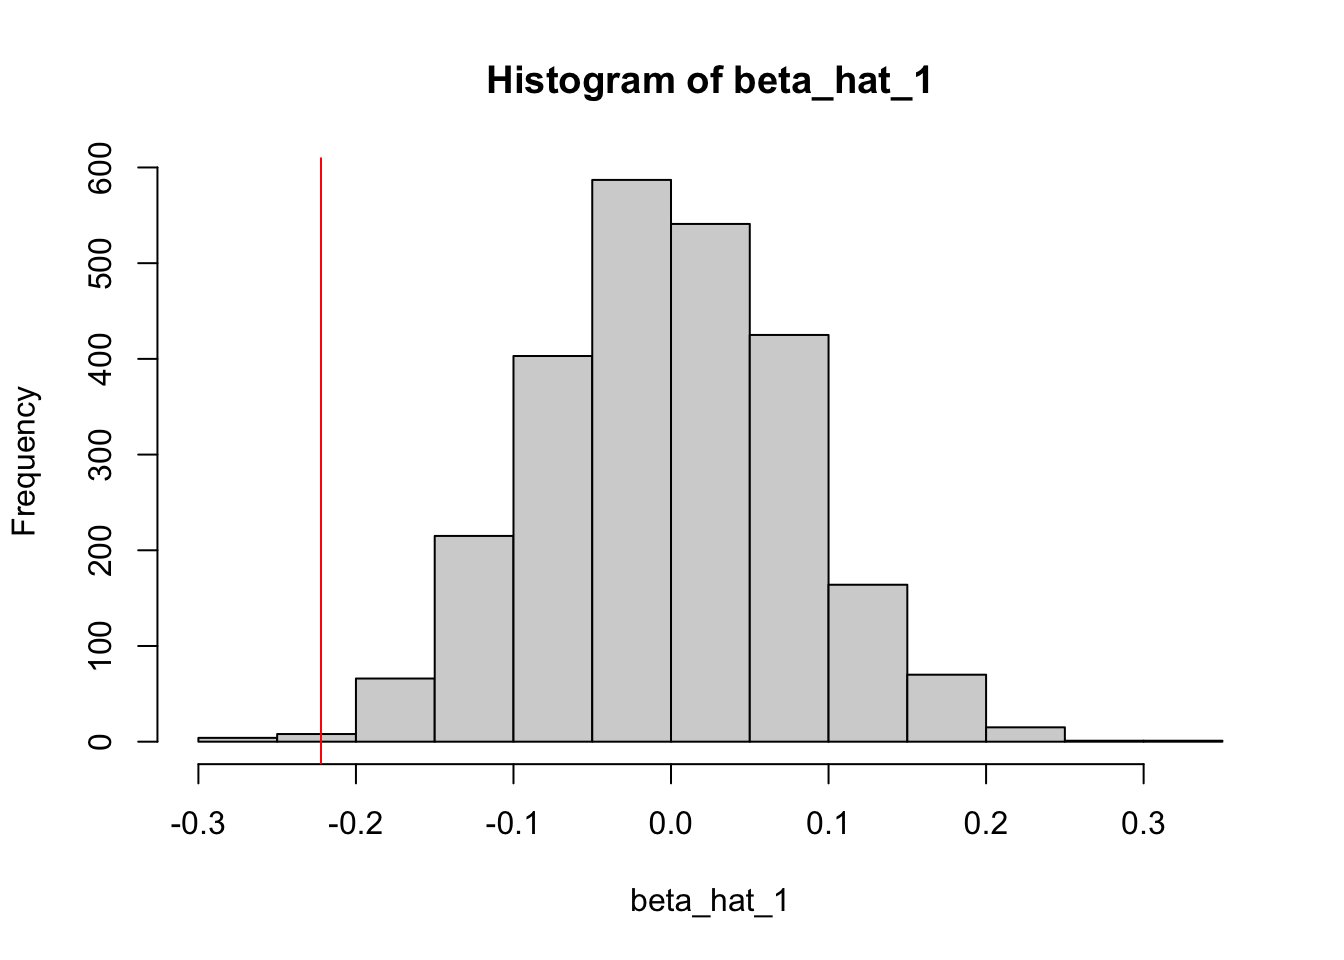
\includegraphics{w02-hw-oboffil2_files/figure-latex/unnamed-chunk-21-1.pdf}

\textbf{(e)} Your value of \(\hat{\beta_1}\) in \textbf{(c)} should be
negative. What proportion of the \texttt{beta\_hat\_1} values is smaller
than your \(\hat{\beta_1}\)? Return this proportion, as well as this
proportion multiplied by \texttt{2}.

\begin{Shaded}
\begin{Highlighting}[]
\NormalTok{proportion =}\StringTok{ }\KeywordTok{sum}\NormalTok{(beta_hat_}\DecValTok{1} \OperatorTok{<}\StringTok{ }\NormalTok{beta_}\DecValTok{1}\NormalTok{_hat_skeptic)}
\NormalTok{proportion}
\end{Highlighting}
\end{Shaded}

\begin{verbatim}
## [1] 7
\end{verbatim}

\begin{Shaded}
\begin{Highlighting}[]
\NormalTok{proportion }\OperatorTok{*}\StringTok{ }\DecValTok{2}
\end{Highlighting}
\end{Shaded}

\begin{verbatim}
## [1] 14
\end{verbatim}

\textbf{(f)} Based on your histogram and part \textbf{(e)}, do you think
the \href{skeptic.csv}{\texttt{skeptic.csv}} data could have been
generated by the model given above? Briefly explain.

The \(\hat{\beta_1}\) is almost the same as the model, this model covers
a good areas of the chart following the empirical rule.

\begin{center}\rule{0.5\linewidth}{0.5pt}\end{center}

\hypertarget{exercise-5-comparing-models}{%
\subsection{Exercise 5 (Comparing
Models)}\label{exercise-5-comparing-models}}

For this exercise we will use the \texttt{Ozone} dataset from the
\texttt{mlbench} package. You should use \texttt{?Ozone} to learn about
the background of this dataset. You may need to install the
\texttt{mlbench} package. If you do so, do not include code to install
the package in your \texttt{R} Markdown document.

For simplicity, we will perform some data cleaning before proceeding.

\begin{Shaded}
\begin{Highlighting}[]
\KeywordTok{data}\NormalTok{(Ozone, }\DataTypeTok{package =} \StringTok{"mlbench"}\NormalTok{)}
\NormalTok{Ozone =}\StringTok{ }\NormalTok{Ozone[, }\KeywordTok{c}\NormalTok{(}\DecValTok{4}\NormalTok{, }\DecValTok{6}\NormalTok{, }\DecValTok{7}\NormalTok{, }\DecValTok{8}\NormalTok{)]}
\KeywordTok{colnames}\NormalTok{(Ozone) =}\StringTok{ }\KeywordTok{c}\NormalTok{(}\StringTok{"ozone"}\NormalTok{, }\StringTok{"wind"}\NormalTok{, }\StringTok{"humidity"}\NormalTok{, }\StringTok{"temp"}\NormalTok{)}
\NormalTok{Ozone =}\StringTok{ }\NormalTok{Ozone[}\KeywordTok{complete.cases}\NormalTok{(Ozone), ]}
\end{Highlighting}
\end{Shaded}

We have:

\begin{itemize}
\tightlist
\item
  Loaded the data from the package
\item
  Subset the data to relevant variables

  \begin{itemize}
  \tightlist
  \item
    This is not really necessary (or perhaps a good idea) but it makes
    the next step easier
  \end{itemize}
\item
  Given variables useful names
\item
  Removed any observation with missing values

  \begin{itemize}
  \tightlist
  \item
    This should be given much more thought in practice
  \end{itemize}
\end{itemize}

For this exercise we will define the ``Root Mean Square Error'' of a
model as

\[
\text{RMSE} = \sqrt{\frac{1}{n} \sum_{i = 1}^{n}(y_i - \hat{y}_i)^2}.
\]

\textbf{(a)} Fit three SLR models, each with ``ozone'' as the response.
For the predictor, use ``wind speed,'' ``humidity percentage,'' and
``temperature'' respectively. For each, calculate \(\text{RMSE}\) and
\(R^2\). Arrange the results in a markdown table, with a row for each
model. Suggestion: Create a data frame that stores the results, then
investigate the \texttt{kable()} function from the \texttt{knitr}
package.

\begin{Shaded}
\begin{Highlighting}[]
\KeywordTok{library}\NormalTok{(}\StringTok{"knitr"}\NormalTok{)}
\NormalTok{fit_wind =}\StringTok{ }\KeywordTok{lm}\NormalTok{(Ozone}\OperatorTok{$}\NormalTok{ozone }\OperatorTok{~}\StringTok{ }\NormalTok{Ozone}\OperatorTok{$}\NormalTok{wind, }\DataTypeTok{data =}\NormalTok{ Ozone)}
\NormalTok{fit_humidity =}\StringTok{ }\KeywordTok{lm}\NormalTok{(Ozone}\OperatorTok{$}\NormalTok{ozone }\OperatorTok{~}\StringTok{ }\NormalTok{Ozone}\OperatorTok{$}\NormalTok{humidity, }\DataTypeTok{data =}\NormalTok{ Ozone)}
\NormalTok{fit_temp =}\StringTok{ }\KeywordTok{lm}\NormalTok{(Ozone}\OperatorTok{$}\NormalTok{ozone }\OperatorTok{~}\StringTok{ }\NormalTok{Ozone}\OperatorTok{$}\NormalTok{temp, }\DataTypeTok{data =}\NormalTok{ Ozone)}

\NormalTok{RMSE =}\StringTok{ }\ControlFlowTok{function}\NormalTok{(error) \{ }\KeywordTok{sqrt}\NormalTok{(}\KeywordTok{mean}\NormalTok{(error}\OperatorTok{^}\DecValTok{2}\NormalTok{)) \}}
\NormalTok{wind_RMSE =}\StringTok{ }\KeywordTok{RMSE}\NormalTok{(fit_wind}\OperatorTok{$}\NormalTok{residuals)}
\NormalTok{humidity_RMSE =}\StringTok{ }\KeywordTok{RMSE}\NormalTok{(fit_humidity}\OperatorTok{$}\NormalTok{residuals)}
\NormalTok{temp_RMSE =}\StringTok{ }\KeywordTok{RMSE}\NormalTok{(fit_temp}\OperatorTok{$}\NormalTok{residuals)}

\NormalTok{R_wind =}\KeywordTok{summary}\NormalTok{(fit_wind)}\OperatorTok{$}\NormalTok{r.squared}
\NormalTok{R_humidity =}\StringTok{ }\KeywordTok{summary}\NormalTok{(fit_humidity)}\OperatorTok{$}\NormalTok{r.squared}
\NormalTok{R_tem =}\StringTok{ }\KeywordTok{summary}\NormalTok{(fit_temp)}\OperatorTok{$}\NormalTok{r.squared}

\NormalTok{df5 =}\StringTok{ }\KeywordTok{data.frame}\NormalTok{(}\StringTok{"Model"}\NormalTok{ =}\StringTok{ }\KeywordTok{c}\NormalTok{(}\StringTok{"Wind:"}\NormalTok{, }\StringTok{"Humidity:"}\NormalTok{, }\StringTok{"Temp:"}\NormalTok{), }\StringTok{"R^2"}\NormalTok{ =}\StringTok{  }\KeywordTok{c}\NormalTok{(R_wind, R_humidity, R_tem), }
           \StringTok{"RMSE"}\NormalTok{ =}\StringTok{ }\KeywordTok{c}\NormalTok{(wind_RMSE, humidity_RMSE, temp_RMSE))}
\KeywordTok{kable}\NormalTok{(df5, }\StringTok{"markdown"}\NormalTok{, }\DataTypeTok{align =} \StringTok{"lrr"}\NormalTok{, }\DataTypeTok{caption =} \StringTok{"Model Table"}\NormalTok{)}
\end{Highlighting}
\end{Shaded}

\begin{longtable}[]{@{}lrr@{}}
\toprule
Model & R.2 & RMSE\tabularnewline
\midrule
\endhead
Wind: & 0.0001402 & 7.961695\tabularnewline
Humidity: & 0.1941105 & 7.147822\tabularnewline
Temp: & 0.6042011 & 5.009257\tabularnewline
\bottomrule
\end{longtable}

\textbf{(b)} Based on the results, which of the three predictors used is
most helpful for predicting ozone readings? Briefly explain.

The Temp Model because it has better \(R^2\) and lower \(\text{RMSE}\)

\begin{center}\rule{0.5\linewidth}{0.5pt}\end{center}

\hypertarget{exercise-00-slr-without-intercept}{%
\subsection{Exercise 00 (SLR without
Intercept)}\label{exercise-00-slr-without-intercept}}

\textbf{This exercise will \emph{not} be graded and is simply provided
for your information. No credit will be given for the completion of this
exercise. Give it a try now, and be sure to read the solutions later.}

Sometimes it can be reasonable to assume that \(\beta_0\) should be 0.
That is, the line should pass through the point \((0, 0)\). For example,
if a car is traveling 0 miles per hour, its stopping distance should be
0! (Unlike what we saw in the book.)

We can simply define a model without an intercept,

\[
Y_i = \beta x_i + \epsilon_i.
\]

\textbf{(a)}
\href{http://daviddalpiaz.github.io/appliedstats/simple-linear-regression.html\#least-squares-approach}{In
the \textbf{Least Squares Approach} section of the text} you saw the
calculus behind the derivation of the regression estimates, and then we
performed the calculation for the \texttt{cars} dataset using
\texttt{R}. Here you need to do, but not show, the derivation for the
slope only model. You should then use that derivation of \(\hat{\beta}\)
to write a function that performs the calculation for the estimate you
derived.

In summary, use the method of least squares to derive an estimate for
\(\beta\) using data points \((x_i, y_i)\) for \(i = 1, 2, \ldots n\).
Simply put, find the value of \(\beta\) to minimize the function

\[
f(\beta)=\sum_{i=1}^{n}(y_{i}-\beta x_{i})^{2}.
\]

Then, write a function \texttt{get\_beta\_no\_int} that takes input:

\begin{itemize}
\tightlist
\item
  \texttt{x} - A predictor variable
\item
  \texttt{y} - A response variable
\end{itemize}

The function should then output the \(\hat{\beta}\) you derived for a
given set of data.

\textbf{(b)} Write your derivation in your \texttt{.Rmd} file using TeX.
Or write your derivation by hand, scan or photograph your work, and
insert it into the \texttt{.Rmd} as an image. See the
\href{http://rmarkdown.rstudio.com/}{RMarkdown documentation} for
working with images.

\textbf{(c)} Test your function on the \texttt{cats} data using body
weight as \texttt{x} and heart weight as \texttt{y}. What is the
estimate for \(\beta\) for this data?

\textbf{(d)} Check your work in \texttt{R}. The following syntax can be
used to fit a model without an intercept:

\begin{Shaded}
\begin{Highlighting}[]
\KeywordTok{lm}\NormalTok{(response }\OperatorTok{~}\StringTok{ }\DecValTok{0} \OperatorTok{+}\StringTok{ }\NormalTok{predictor, }\DataTypeTok{data =}\NormalTok{ dataset)}
\end{Highlighting}
\end{Shaded}

Use this to fit a model to the \texttt{cat} data without an intercept.
Output the coefficient of the fitted model. It should match your answer
to \textbf{(c)}.

\end{document}
